\documentclass{haskellbeamer}

\title{Solving Data-flow Problems in Syntax Trees}
\date{September 9, 2017}

\input{defs.tex}

\begin{document}

\maketitle

\begin{frame}{Introduction}
  \begin{itemize}
    \item My master's thesis\footnote{\tiny\url{https://pp.ipd.kit.edu/uploads/publikationen/graf17masterarbeit.pdf}}: Call Arity vs. Demand Analysis
      \begin{itemize}
        \item Result: Usage Analysis generalising Call Arity
        \item Precision of Call Arity without co-call graphs
      \end{itemize}
    \item Requirements led to complex analysis order
    \item \emph{Specification} of data-flow problem decoupled from its \emph{solution}
  \end{itemize}
\end{frame}

\begin{frame}[fragile]{Strictness Analysis}
  \begin{itemize}
    \item Provides lower bounds on \emph{evaluation cardinality}
    \item Which variables are evaluated at least once?
      \begin{itemize}
        \item[$S$] Strict (Yes!)
        \item[$L$] Lazy (Not sure)
      \end{itemize}
    \item Enables call-by-value, unboxing
  \end{itemize}
  \begin{overprint}
    \onslide<1>
    \begin{center}
      \begin{minipage}{0.5\textwidth}
        \begin{haskell}
          main = do
            let  x = ... -- $S$
            let  y = ... -- $S$
            let  z = ... -- $L$
            print (x + if odd y then y else z)
        \end{haskell}
      \end{minipage}
    \end{center}
    \onslide<2>
    \begin{center}
      \begin{minipage}{0.5\textwidth}
        \begin{haskell}
          main = do
            let !x = ... -- $S$
            let !y = ... -- $S$
            let  z = ... -- $L$
            print (x + if odd y then y else z)
        \end{haskell}
      \end{minipage}
    \end{center}
  \end{overprint}
\end{frame}

\begin{frame}[fragile]{GHC's Demand Analyser}
  \begin{itemize}
    \item Performs strictness analysis (among other things)
    \item Fuels Worker/Wrapper transformation
    \item Backward analysis
      \begin{itemize}
        \item Which strictness does an expression place on its free variables?
        \item Which strictness does a function place its arguments?
      \end{itemize}
    \item \emph{Strictness type}: $\sStrType = \lPair{\sFVs \pfun \sStr}{\sStr^*}$
  \end{itemize}
\end{frame}

\begin{frame}[fragile]{Strictness Signatures}
  \begin{itemize}
    \item Looks at the right-hand side of \hs{const} before the \hs{let} body!
    \item \emph{Unleashes} strictness type of \hs{const}'s RHS at call sites
  \end{itemize}
  \begin{center}
    \begin{minipage}{0.8\textwidth}
      \begin{haskell}
        let const a b = a -- $\mathtt{const} :: \lPair{\emptymap}{[S, L]}$
        in const 
            y             -- $S$
            (fac 1000)    -- $L$
      \end{haskell}
    \end{minipage}
  \end{center}
\end{frame}

\begin{frame}[fragile]{Call Context Matters}
  \begin{overprint}
    \onslide<1-3>
    \begin{itemize}
      \item Whole expression is strict in \hs{z}
      \item Only digests \hs{f} for manifest arity 1, can't look under lambda
      \item \hs{f} is called with 2 arguments
      \item<4>[\ding{213}] Analyse bound function when incoming arity is known
    \end{itemize}
    \onslide<4->
    \begin{itemize}
      \item Solution: Analyse RHS when incoming arity is known
      \item Formally: Finite approximation of \emph{strictness transformer}
        \begin{itemize}
          \item $\sStrTrans = \mathbb{N} \to \sStrType$
        \end{itemize}
      \item Exploit laziness to memoise results?
    \end{itemize}
  \end{overprint}
  \begin{overprint}
    \onslide<1>
    \begin{center}
      \begin{minipage}{0.7\textwidth}
        \begin{haskell*}{escapeinside=||}
          let f x = -- $\mathtt{f} :: \lPair{\maplit{\mathtt{z}}{L}}{[S]}$
                if odd x
                  then \y -> y*|\color{red}\texttt{z}|
                  else \y -> y+|\color{red}\texttt{z}|
          in f 1 2
        \end{haskell*}
      \end{minipage}
    \end{center}
    \onslide<2>
    \begin{center}
      \begin{minipage}{0.7\textwidth}
        \begin{haskell*}{escapeinside=||}
          let f x = -- $\mathtt{f} :: \lPair{\maplit{\mathtt{z}}{L}}{[S]}$
                if odd x
                  then \y -> y*|\color{red}\texttt{z}|
                  else \y -> y+|\color{red}\texttt{z}|
          in seq (f 1) 42
        \end{haskell*}
      \end{minipage}
    \end{center}
    \onslide<3>
    \begin{center}
      \begin{minipage}{0.7\textwidth}
        \begin{haskell*}{escapeinside=||}
          let f x = -- $\mathtt{f} :: \lPair{\maplit{\mathtt{z}}{L}}{[S]}$
                if odd x
                  then \y -> y*z
                  else \y -> y+z
          in f 1 2
        \end{haskell*}
      \end{minipage}
    \end{center}
    \onslide<4>
    \begin{center}
      \begin{minipage}{0.7\textwidth}
        \begin{haskell*}{escapeinside=||}
          let f x = -- $\mathtt{f}_{\color{red}1} :: \lPair{\maplit{\mathtt{z}}{L}}{[S]}$
                if odd x
                  then \y -> y*z
                  else \y -> y+z
          in f 1 2
        \end{haskell*}
      \end{minipage}
    \end{center}
    \onslide<5>
    \begin{center}
      \begin{minipage}{0.7\textwidth}
        \begin{haskell*}{escapeinside=||}
          let f x = -- $\mathtt{f}_{\color{red}2} :: \lPair{\maplit{\mathtt{z}}{S}}{[S,S]}$
                if odd x
                  then \y -> y*z
                  else \y -> y+z
          in f 1 2
        \end{haskell*}
      \end{minipage}
    \end{center}
  \end{overprint}
\end{frame}
  
\begin{frame}[fragile]{Recursion}
  \begin{itemize}
    \item Exploit laziness to memoise approximations?
    \item[\xmark] Recursion leads to termination problems
    \item Rediscovered fixed-point iteration, detached from the syntax tree
    \item Leads to data-flow network, solved by worklist algorithm
  \end{itemize}
  \begin{center}
    \begin{minipage}{0.5\textwidth}
      \begin{haskell}
        let fac n = 
              if n == 0
                then 1
                else n * fac (n-1)
        in fac 12
      \end{haskell}
    \end{minipage}
  \end{center}
\end{frame}

\begin{frame}[fragile]{Example}
  \begin{itemize}
    \item Allocate one top-level node + one node per \hs{let} binding
  \end{itemize}
  \begin{columns}
    \begin{column}{0.35\textwidth}
      \begin{haskell}
        let even 0 = True
            even n = odd (n-1)
            odd 0 = False
            odd n = even (n-1)
        in even 12
      \end{haskell}
    \end{column}
    \begin{column}{0.05\textwidth}
      {\Huge$\Rightarrow$}
    \end{column}
    \begin{column}{0.35\textwidth}
      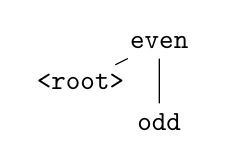
\begin{tikzpicture}
        \node at (0,0) (root) {\texttt{<root>}};
        \node at (1,0.5) (even) {\texttt{even}};
        \node at (1,-0.5) (odd) {\texttt{odd}};
        \draw (root) -> (even) -- (odd);
      \end{tikzpicture}
    \end{column}
  \end{columns}
    
\end{frame}

\section{End}
\end{document}